\subsection{DATA SHEET \#1} 

	\item Calculate the time constant for the circuit with the above values of R and C.\\
		
		RC = 0.00015 seconds
	\item Record the frequency reading from the function generator.\\
	
		Calculate the period T for this wave: 600.3 Hz \\
		
	\item Record your vertical (VOLTS/DIV) and horizontal settings (TIME/DIV) for the capacitor channel CH2 in the boxes below.
	
		VOLTS/DIV = 1 V\\
		
		TIME/DIV = 0.5 ms.
	\begin{samepage}
	\item Draw carefully what you observe on the screen for the capacitor response at these settings.\\
	
		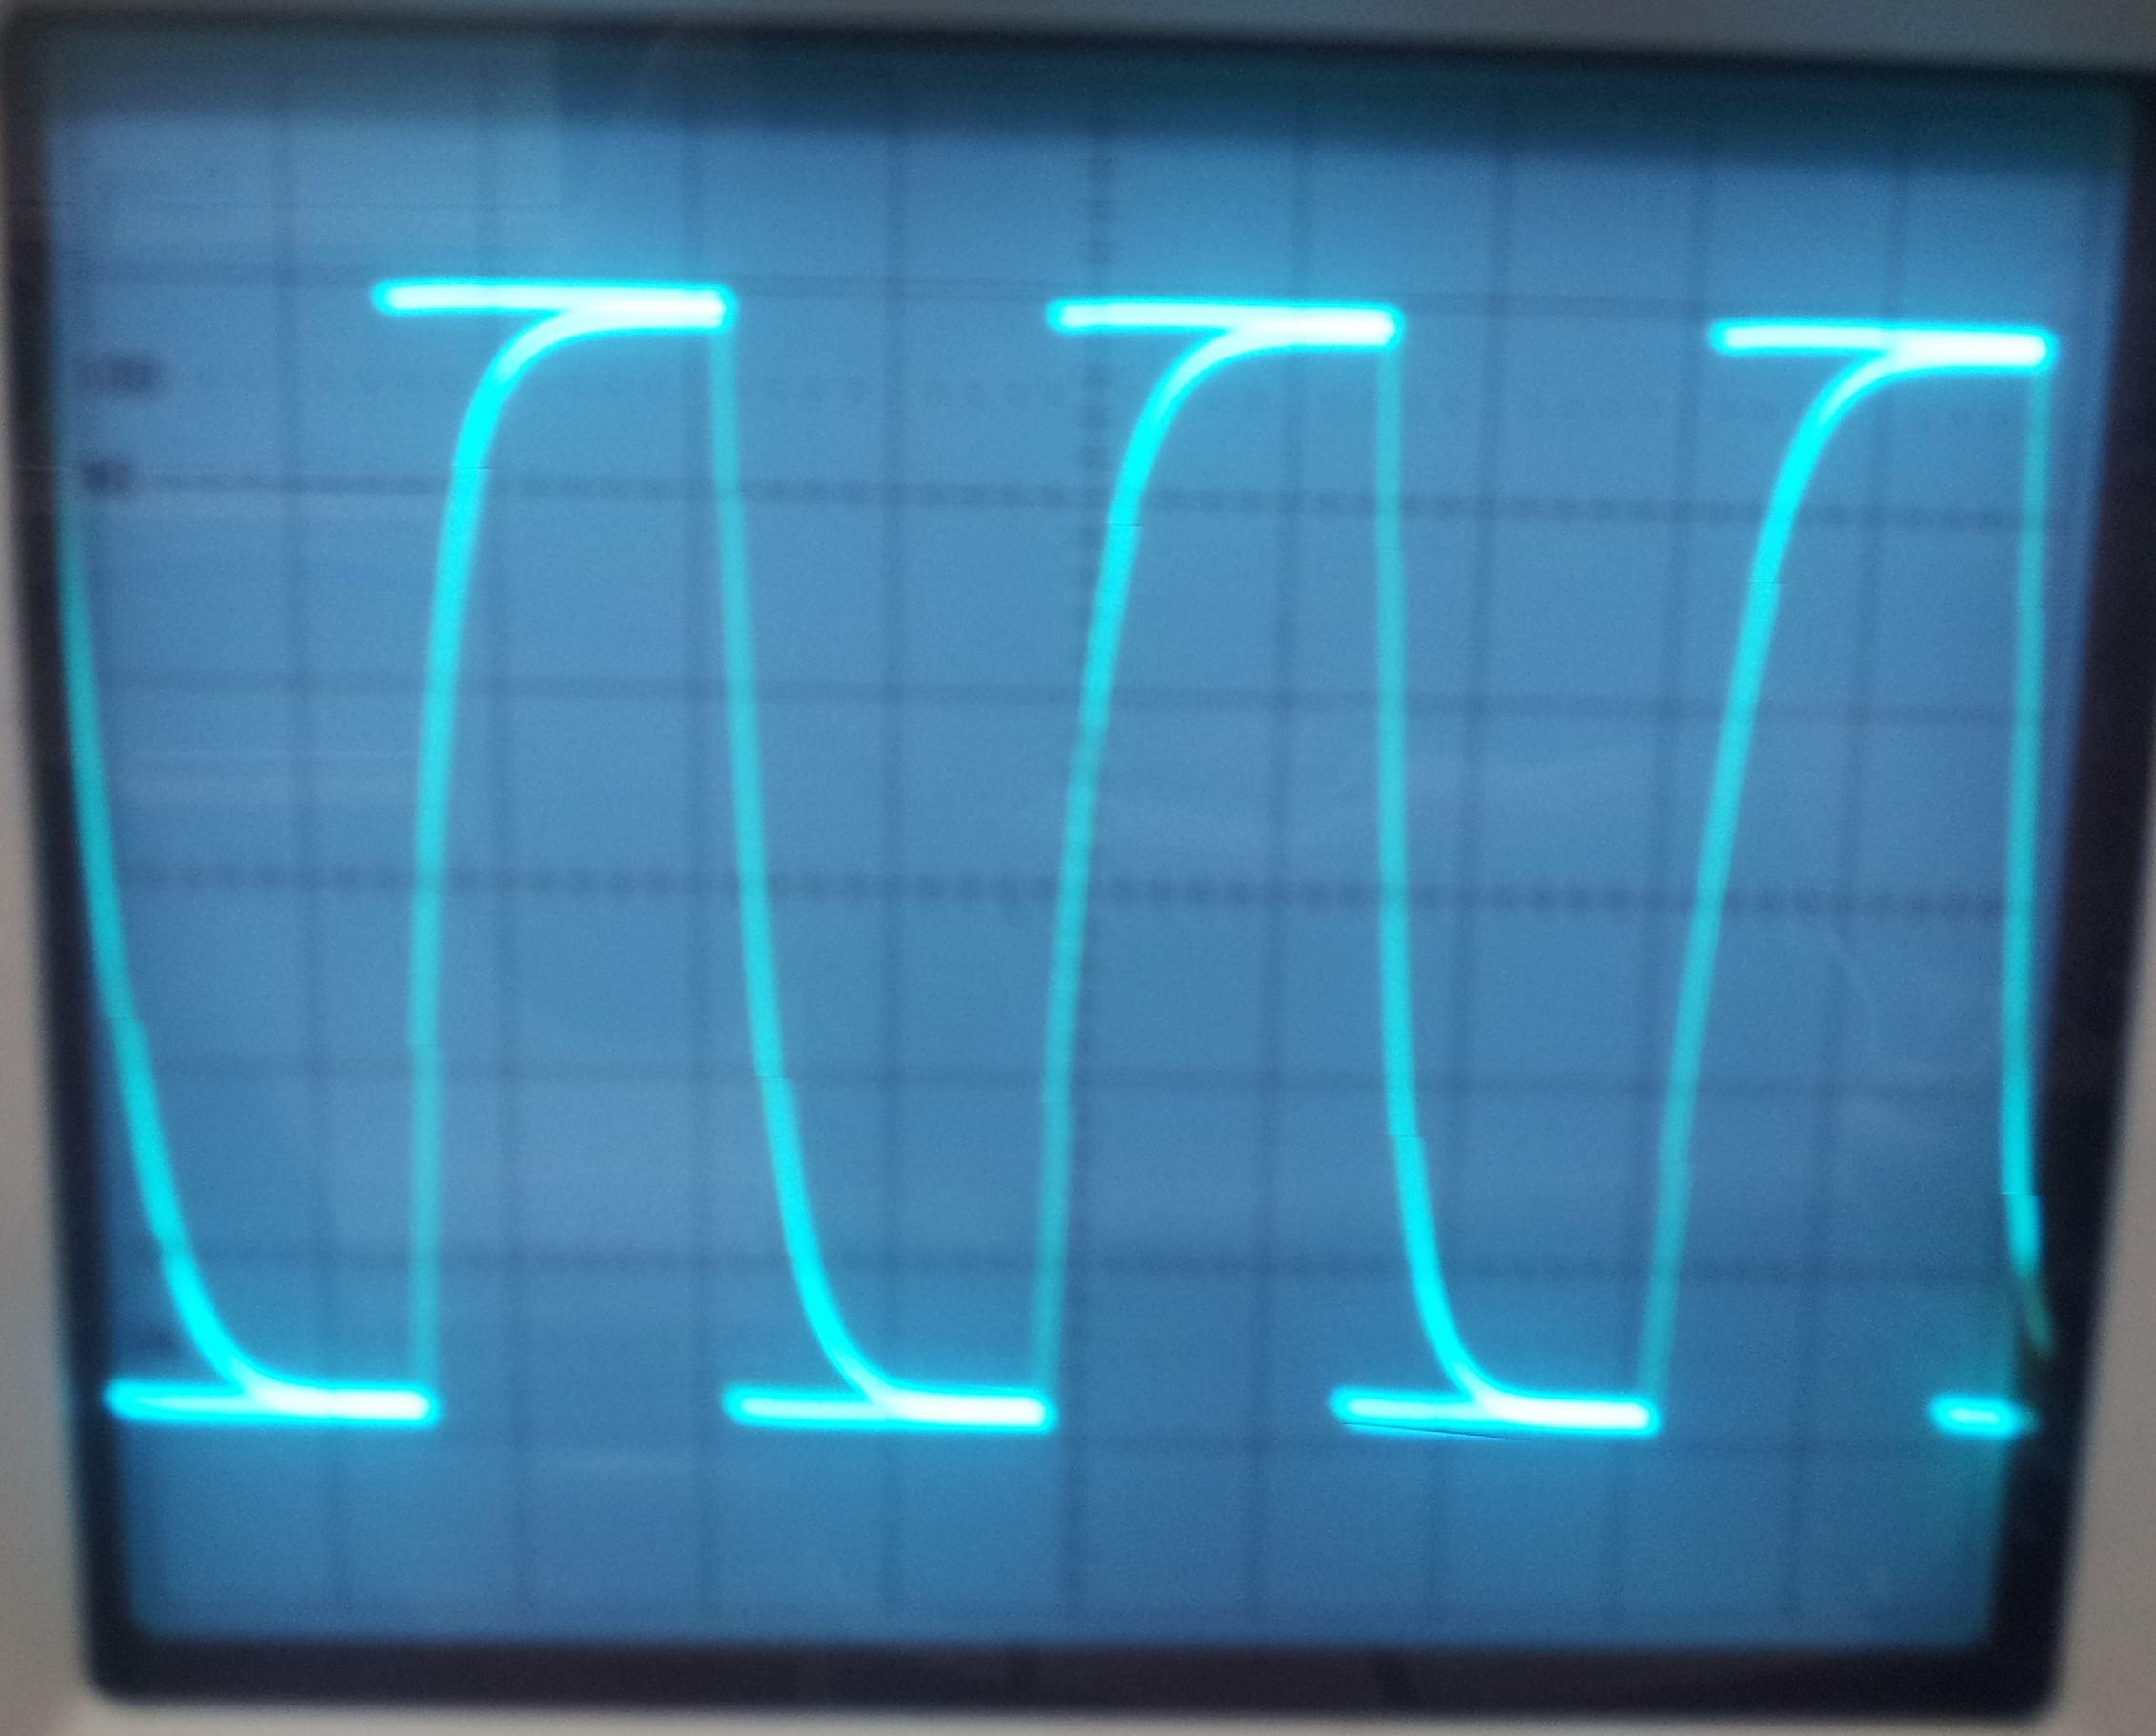
\includegraphics[width=300px]{lab8_graph1}
	\end{samepage}
	\item From the screen, what is the charging time for the capacitor in one cycle?\\
	
		1.5 divisions or about 0.8 ms.\\
	
	\item State how the screen image of a charging cycle is consistent or not with the time constant of this circuit.  Is the charging cycle much longer or much shorter than RC?\\
	
		The charging time is about 0.7 ms shorter on the screen than we calculated above.
	
		